\documentclass[12pt]{report}
\usepackage{../mystyle}
\begin{document}
\newcommand{\HRule}{\rule{\linewidth}{0.5mm}}

\begin{titlepage}

\centering
	
\includegraphics[width=0.2\textwidth]{./title/logohse.png}\par\vspace{1cm}
	{\scshape \LARGE Higher School of Economics \\ \small(National Research University)\par}
	{\scshape \Large Faculty of Computer Science\par}
	\vspace{3cm}
	{\scshape\Large Home Assignment \par \Large{Course: ``Modern Methods of Data Analysis''}\par}
%	\vspace{1cm}
    \HRule \\[0.5cm]
    { \Large \bfseries Medium Articles Analysis}\\[0.2cm] % Title of your document
    \HRule
	\vspace{3.5cm}
	\begin{flushright}
	Student: Ryabykin Alexey \\
	Professor: Ignatov Dmitriy Igorevich
	\\
	Grade: \underline{\hspace{0.2cm}}
    \end{flushright}
    \vfill

	{\large Moscow, 2022}
\end{titlepage}
\boldmath
\tableofcontents
\newpage
\pagestyle{fancy}

\fancyhead[L]{Домашнее задание 1}
\fancyhead[C]{\currentname}
\fancyhead[R]{Рябыкин Алексей}

\section{Постановка задачи}
\par 
\emph{Выбранные данные:} Российский мониторинг экономического положения и здоровья населения НИУ ВШЭ (\href{https://www.hse.ru/rlms/spss}{RLMS-HSE}).
\par
Этапы работы:
\begin{enumerate*}
    \item Произвести предварительный анализ выбранных количественных признаков на основе расчета для каждого из них базовых выборочных характеристик (статистик) центральной тенденции и разброса: квантилей, моды, среднего значения, дисперсии и среднего квадратического отклонения. Построить непараметрическую модель эмпирического распределения для одного из количественных признаков;
    \item Проанализировать репрезентативность выборки и определить возможность использования различных методов ее коррекции: определить доли и структуру пропущенных значений и их возможное влияние на статистические выводы. Предложить меры работы с данными, содержащими пропуски и экстремальные значения. Исследовать возможность корректировки выборки с целью обеспечения репрезентативности путем перевзвешивания наблюдений;
    \item Построить доверительные интервалы для параметров генеральной совокупности на основе выборочных данных: генерального среднего и генеральной дисперсии для каждого из количественных признаков и генеральной доли для каждого из качественных признаков;
    \item Произвести проверку гипотез о значениях некоторых параметров генеральной совокупности, например, о равенстве значений признака для определенных групп населения, о соответствии значения признака некоторому декларируемому уровню;
    \item Проанализировать взаимосвязь между признаками, характеризующими исследуемые объекты, и определить ее значимость. Сформулировать выводы по результатам проведенного исследования.
\end{enumerate*}
\par
\emph{Целью исследования} можно назвать формирование понимания и формализацию закономерностей в финансовой и имущественной обеспеченности населения России.
\par 
\emph{Регионом исследования} был выбран Москва.
\newpage
\section{Описание данных и выбранных признаков}
\par
Доходы, исходя из данных и международных принципов их дифференциации, могут быть представлены следующими видами:
\begin{table}[H]
    \centering
    \begin{tabular}{|l|l|}
        \hline
        Доходы                                                  & Виды доходов в исследовании            \\ \hline
        \multicolumn{1}{|c|}{\multirow{4}{*}{Первичные доходы}} & Оплата труда                           \\ \cline{2-2} 
        \multicolumn{1}{|c|}{}                                  & Продажа сельскохозяйственной продукции \\ \cline{2-2} 
        \multicolumn{1}{|c|}{}                                  & Личное хозяйство                       \\ \cline{2-2} 
        \multicolumn{1}{|c|}{}                                  & Предпринимательская деятельность       \\ \hline
        \multirow{2}{*}{Собственность}                          & Аренда недвижимости                    \\ \cline{2-2} 
                                                                & Проценты                               \\ \hline
        \multirow{6}{*}{Трансферты}                             & Пенсии                                 \\ \cline{2-2} 
                                                                & Стипендии                              \\ \cline{2-2} 
                                                                & Пособия                                \\ \cline{2-2} 
                                                                & Алименты                               \\ \cline{2-2} 
                                                                & Пособия по безработице                 \\ \cline{2-2} 
                                                                & Другие доходы                          \\ \hline
        \multirow{2}{*}{Прочие поступления}                     & Продажа личного имущества              \\ \cline{2-2} 
                                                                & Продажа недвижимости                   \\ \hline
        \end{tabular}
\caption{Доходы и их виды}
\end{table}
\par
С другой стороны, среди расходов и имуществ населения можно выделить следующие группы для анализа:

\begin{table}[H]
    \parbox{0.45\linewidth}{\begin{tabular}{|l|l|}
    \hline
    Расходы                 & Примеры                     \\ \hline
    Потребительские расходы & Продукты питания            \\ \hline
    Платежи и взносы        & Налоги, связь, интернет     \\ \hline
    Приобретение имущества  & Квартиры, гараж и прочее    \\ \hline
    Денежные сбережения     & Вклады, сбережения в валюте \\ \hline
    \end{tabular}
    \caption{Расходы и их виды}
    } \hspace*{2cm}
       \parbox{0.45\linewidth}{\begin{tabular}{|l|l|}
        \hline
        Активы            & Примеры                \\ \hline
        Реальные активы   & Квартира, дача, машина \\ \hline
        Оборотные активы  & Одежда, наличные       \\ \hline
        Финансовые активы & Арендное имущество     \\ \hline
        \end{tabular}
        \caption{Типы имущества}
        }
\end{table}
Для анализа были выбраны более-менее заполненные данные, связанные с представленными ранее.

\section{Предварительный анализ данных}
Данные содержат результаты опроса 413 респондентов из Москвы по практически 1.5 тысячам вопросам различного характера. 
\begin{longtable}{llcc}
  \toprule
   Столбец &                                                                                             Описание &  Количество п.з. & Доля п. з. \\
  \midrule
  \endfirsthead
  
  \toprule
   Столбец &                                                                                             Описание &  Количество п. з. & Доля п. з. \\
  \midrule
  \endhead
  \midrule
  \multicolumn{4}{r}{{Продолжение на следующей странице}} \\
  \midrule
  \endfoot
  
  \bottomrule
  \endlastfoot
     z\_nfm &                                                                              Количество членов семьи &                                0 &                      0.0\% \\
     zc1.1 &                                  Стоимость Вашего жилья? &                                0 &                      0.0\% \\
       zc6 & Полезная площадь Вашего жилья? &                                0 &                      0.0\% \\
       zc5 & Жилая площаль Вашего жилья? &                                0 &                      0.0\% \\
  zc9.7.2a &                                                         В наличии отечественный легковой автомобиль &                                0 &                      0.0\% \\
  zc9.7.3a &                                                  В наличии легковой автомобиль иностранной модели?  &                                0 &                      0.0\% \\
  zc9.7.1a &                                                                      В наличии грузовой автомобиль? &                                0 &                      0.0\% \\
    zc9.8a &                                                     В наличии мотоцикл, мотороллер, моторная лодка? &                                0 &                      0.0\% \\
  zc9.101a &                                           В наличии дача или другой дом, садовый домик? &                                0 &                      0.0\% \\
   zc9.12a &                                                       В наличии другая квартира или часть квартиры? &                                0 &                      0.0\% \\
    ze1.1c &                  Траты за 7 дней на белый хлеб &                               57 &                     13.8\% \\
       ze4 & Траты на еду &                                0 &                      0.0\% \\
    ze9.8b &                        Траты на оплату мобильной связи  &                               13 &                      3.1\% \\
      ze11 & Траты на квартиру (коммунальные, аренда) &                               16 &                      3.9\% \\
      ze12 &             Наличие задолженностей по квартире? &                                0 &                      0.0\% \\
      ze44 &                                                   Практикуют раздельный сбор мусора? &                                0 &                      0.0\% \\
      ze14 &                                         Ваша семья в течение 30 дней давала деньги в долг? &                                0 &                      0.0\% \\
      ze16 &                                       Ваша семья в течение 30 дней откладывала сбережения? &                                0 &                      0.0\% \\
    zf12\_a & Как долго смогли бы жить только за счет сбережений? &                                0 &                      0.0\% \\
    zf14.8 &                                   Долги по кредитам &                                0 &                      0.0\% \\
   zf14.12 &                                                                               Должны ли Вашей семье? &                                0 &                      0.0\% \\
      zf14 &                                                                                       Денежный доход &                                0 &                      0.0\% \\
    \caption{Доля пропущенных значений}
  \end{longtable}
\begin{note}{}
    Описание некоторых столбцов здесь и впредь было изменено для адекватного отображения таблиц, рисунков, диаграмм.
  \end{note}
  \par
  Среди выбранных признаков доля пропущенных значений не очень велика, заполнение для категориальных возможно с помощью категориальных значений ``ОТКАЗ ОТ ОТВЕТА'', ``НЕТ ОТВЕТА''. Их природа (как пропусков, так и перечисленных категориальных значений) может лежать в неуверенности респондентов в ответе или в нежелании разглашать личную информацию. 
  
  \par
  Проведем предварительный анализ выбранных количественных признаков, рассчитав для каждого выборочные характеристики центральной тенденции и разброса:
  \begin{table}[H]
    \begin{tabular}{|l|p{3cm}|c|c|c|c|c|c|}
    \hline
    Признак & Описание                   & $q_{25}$ & $q_{75}$ & mean      & mode     & std       & variance       \\ \hline
    z\_nfm  & Количество членов семьи    & 1        & 4        & 2.56      & 1        & 1.5       & 2.26           \\ \hline
    zc6     & Полезная площадь           & 42.4     & 60.225   & 53.24     & 52       & 15.4      & 237.2          \\ \hline
    ze11    & Квартплата (+коммунальные) & 5000     & 8000     & 7021      & 7000     & 3814.8    & 14552570       \\ \hline
    zc5     & Площадь квартиры (жилая)   & 26.375   & 42       & 34        & 30       & 12        & 148            \\ \hline
    ze1.1   & Примерная стоимость жилья  & 6750000  & 12000000 & 9478285.7 & 10000000 & 3941801.8 & 15537801642036 \\ \hline
    ze1.1c  & Траты на белый хлеб        & 45       & 122      & 105       & 40       & 90.5      & 8182.5         \\ \hline
    ze4     & Траты на питание           & 15000    & 30000    & 23309     & 20000    & 12910.2   & 166673104.7    \\ \hline
    ze9.8b  & Траты на мобильную связь   & 500      & 1500     & 1195.6    & 1000     & 1300.7    & 1691897.7      \\ \hline
    zf14    & Денежный доход             & 43000    & 117225   & 88354     & 50000    & 67447.5   & 4549163351     \\ \hline
    \end{tabular}
    \caption{Базовые выборочные характеристики для количественных признаков}
    \end{table}
    \par
    Построим распределение для доходов и расходов. Как доходы, так и расходы есть совокупность денежных средств, полученных из различных источников или затраченных на различные цели. Поэтому распределение трат (или доходов) домохозяйств может иметь вид аддитивной смеси распределений. Предположим, что закон распределения расходов будет смесью логарифмически-нормальных распределений:
    \useshortskip
    \[
        f(\ln y) = \sum\limits_{i=1}^n q_i f(\ln y, \mu_i, \sigma_i),
    \] 
    \useshortskip
    где $n$ -- предполагаемое количество групп, $q_i$ -- доля объектов $i$-й группы, причем $\sum\limits_{i=1}^n q_i = 1$. Построим эмпирическое распределение логарифма затрат:
    \begin{figure}[H]
      \centering
      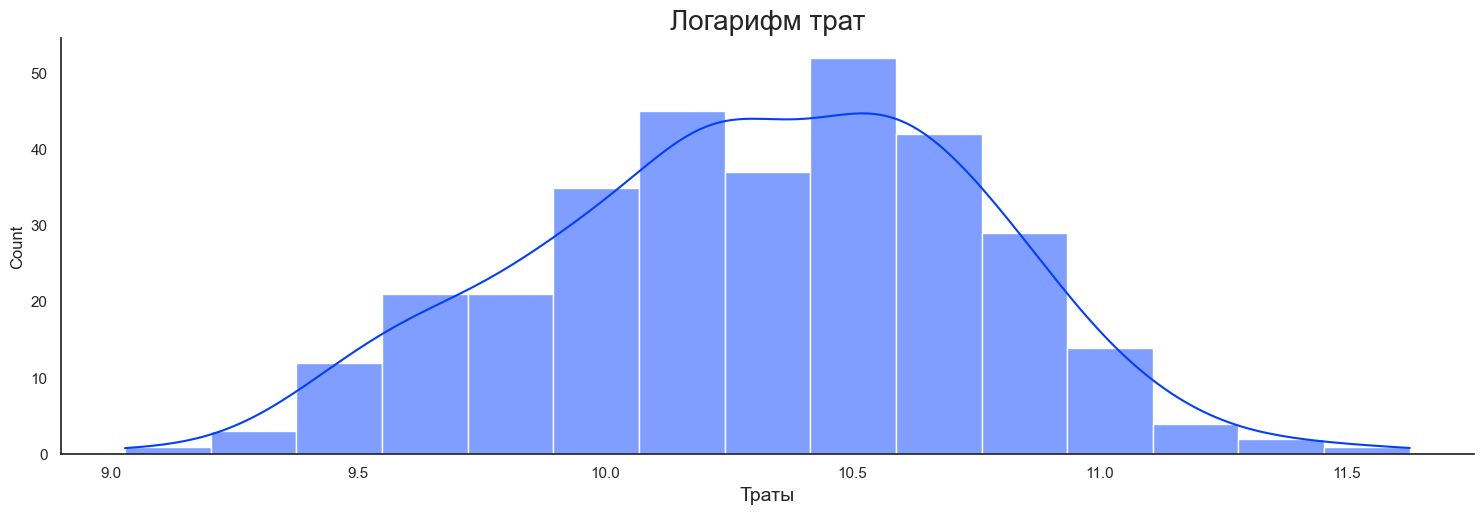
\includegraphics[scale=0.5]{title/outcome.png}
      \caption{Гистограмма эмпирического распределения логарифма затрат}
    \end{figure}
    По критерию Шапиро-Уилка логарифм затрат подчиняется нормальному закону распределения на уровне значимости $0.1$.
    Так же можно посмотреть на распределения по типам затрат:
    \begin{figure}[H]
      \centering
      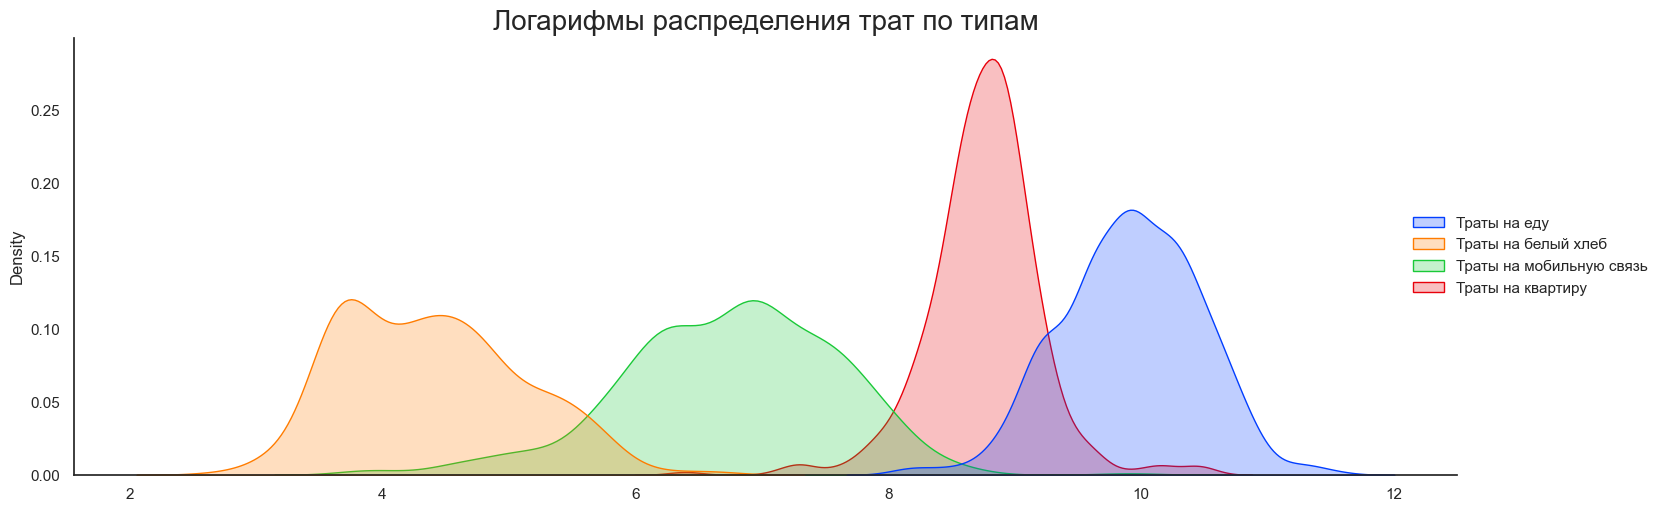
\includegraphics[scale=0.45]{title/outcome_different.png}
      \caption{Распределения логарифмов затрат для разных категорий}
    \end{figure}
    \par
    Видим колокообразные распределения затрат для домохозяйств. Для количественных данных пропуски можно заполнить средними значениями, например, для расходов, средними разного рода (математическим ожиданием, модой, медианой), для площади квартиры или стоимости квартиры (пропущенных значений нет, однако иногда респонденты отвечали в соответствии с перечисленными категориальными значениями) так же можно заполнить средними или выделить схожие группы по площади для заполнения стоимости. 

    {\begin{wrapfigure}[16]{r}{0.25\columnwidth}
      \vspace*{-0.5cm}
      \begin{flushright}
        \hspace*{-0.5cm} 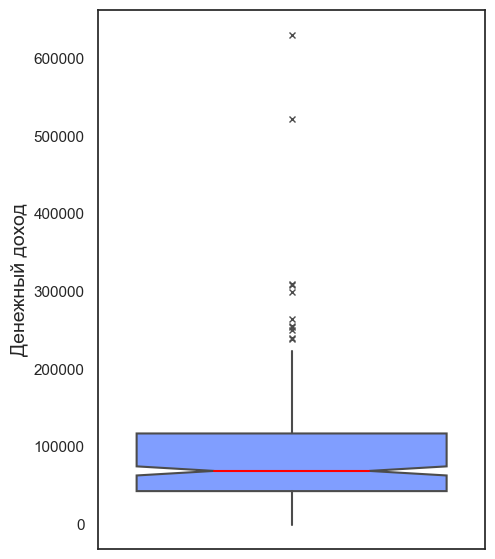
\includegraphics[scale=0.45]{title/income_with_bad_values.png}  
        \caption{Ящик с усами для доходов}      
      \end{flushright}
    \end{wrapfigure}
    \par
    Для дохода можем наблюдать значительные выбросы. Природа этих выбросов может зависеть от двух аспектов. Первый: неравенство доходов, зиждящееся на банальном социальном неравенстве, при котором присутствуют люди, зарабатывающие сильно больше прочих. С другой стороны, это может быть обман  респондентов с различными целями (от поднятия эго до умышленного искажения информации, например, для поднятия среднего заработка). 
    \par
    Избавимся от выбросов и построим распределение денежных доходов. При-\\меним фильтр Хэмпеля, который избавляется от значений, у которых разница с \\медианой больше, чем три медианных абсолютных отклонения.}

    \begin{figure}[H]
      \hspace*{2cm}
      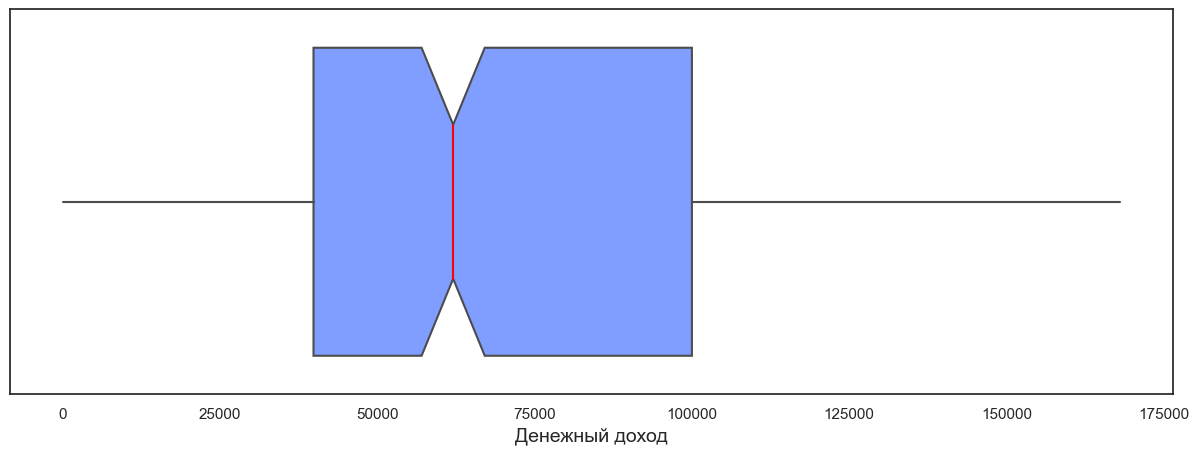
\includegraphics[scale=0.3]{title/income_boxplot.png}
      \captionsetup{oneside,margin={-16cm,-10cm}}
       \caption{Ящик с усами после избавления от выбросов}
    \end{figure}
    Теперь можем построить распределение доходов для населения:
    \begin{figure}[H]
      \centering
      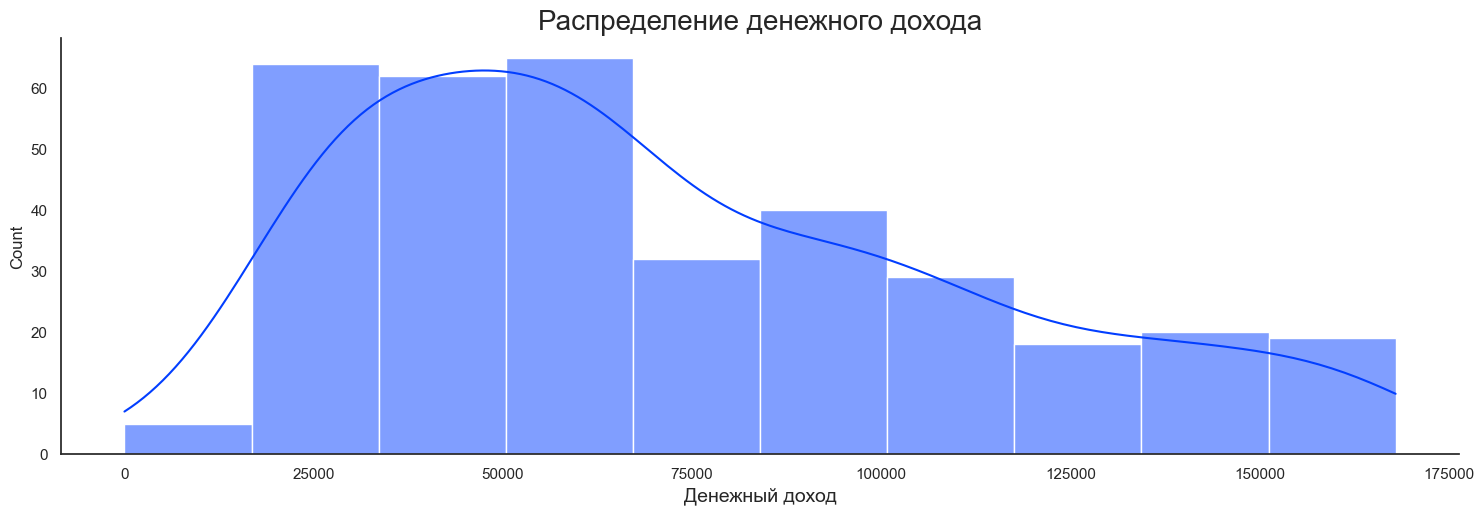
\includegraphics[scale=0.5]{title/income.png}
      \caption{Гистограмма эмпирического распределения денежного дохода}
    \end{figure}
    \par
    О нормальности распределения речи не идет. Стоит отметить, что эти данные точно не репрезантативны для целой страны, особенно беря во внимание показатели минимального размера оплаты труда по Российской Федерации. Однако данные репрезентативны для выбранного региона.
    \par
    Наличие значений признаков вида ``ЗАТРУДНЯЮСЬ ОТВЕТИТЬ'' или ``НЕТ ОТВЕТА'' сильно сказывается на репрезентативности. Предположение по поводу сущности их бытия было выше. К счастью, такие значения составляют малую долю ответов респондентов, поэтому решением было просто их опустить (особенно относительно количественных признаков). Для категориальных данных особенно поддается объяснению в виде нежелания разглашать личную информацию признак ``Наличия сбережений'', в котором их содержится больше, чем в остальных столбцах.
    \newpage
    Посмотрим на категориальные переменные. Построим \emph{pie-plots} для каждой.
    \begin{figure}[H]
      
\includegraphics[scale=0.3]{./title/output.png}
      \caption{Распределение ответов для категориальных переменных}
    \end{figure}
\section{Доверительные интервалы для параметров генеральной совокупности}
\par
Построим доверительные интервалы для параметров генеральной совокупности. Так как наша выборка достаточно большая, то будем пользоваться $t$-статистикой Стьюдента для оценки генерального среднего для количественных признаков. Тогда доверительный интервал будет иметь вид:
\[
    \left(\overline{x} - t_{\alpha} \dfrac{s}{\sqrt{n-1}}, \overline{x} + t_\alpha \dfrac{s}{\sqrt{n-1}}\right)
\]
Для оценки генеральной дисперсии доверительный интервал будет иметь вид:
\[
    \left(\dfrac{s^2(n-1)}{\chi^2_{1-\frac{\alpha}{2}, n-1}}, \dfrac{s^2(n-1)}{\chi^2_{\frac{\alpha}{2}, n-1}}\right)
\]
Доверительные интервалы для генерального среднего количественных величин:
\begin{table}[H]
  \begin{tabular}{|l|l|l|l|l|l|}
  \hline
  Признак & Описание                   & \begin{tabular}[c]{@{}l@{}}Левая \\ граница \\ (для $\alpha = 0.95$)\end{tabular} & \begin{tabular}[c]{@{}l@{}}Правая \\ граница\\ (для $\alpha = 0.95$)\end{tabular} & \begin{tabular}[c]{@{}l@{}}Левая \\ граница \\ (для $\alpha = 0.99$)\end{tabular} & \begin{tabular}[c]{@{}l@{}}Правая \\ граница\\ (для $\alpha = 0.99$)\end{tabular} \\ \hline
  z\_nfm  & Количество членов семьи    & 2.41                                                                              & 2.7                                                                               & 2.37                                                                              & 2.75                                                                              \\ \hline
  zc6     & Полезная площадь           & 51.74                                                                             & 54.73                                                                             & 51.3                                                                              & 55.2                                                                              \\ \hline
  ze11    & Квартплата (+коммунальные) & 6646                                                                              & 7396                                                                              & 6528                                                                              & 7514.6                                                                            \\ \hline
  zc5     & Площадь квартиры (жилая)   & 32.9                                                                              & 35.23                                                                             & 32.5                                                                              & 35.6                                                                              \\ \hline
  ze1.1   & Примерная стоимость жилья  & 8894270.9                                                                         & 10062300.5                                                                        & 8710760                                                                           & 10245811                                                                          \\ \hline
  ze1.1c  & Траты на белый хлеб        & 95.5                                                                              & 114.4                                                                             & 92.5                                                                              & 117.4                                                                             \\ \hline
  ze4     & Траты на питание           & 22042.5                                                                           & 24576                                                                             & 21644.5                                                                           & 24974                                                                             \\ \hline
  ze9.8b  & Траты на мобильную связь   & 1067.35                                                                           & 1323.9                                                                            & 1027                                                                              & 1364.2                                                                            \\ \hline
  zf14    & Денежный доход             & 81711                                                                             & 94997                                                                             & 79624                                                                             & 97084.5                                                                           \\ \hline
  \end{tabular}
  \caption{Доверительные интервалы для генерального среднего}
  \end{table}
  Доверительные интервалы для генеральной дисперсии количественных величин:
  \begin{table}[H]
    \begin{tabular}{|l|p{3cm}|l|l|l|l|}
    \hline
    Признак & Описание                   & \begin{tabular}[c]{@{}l@{}}Левая \\ граница \\ (для $\alpha = 0.05$)\end{tabular} & \begin{tabular}[c]{@{}l@{}}Правая \\ граница\\ (для $\alpha = 0.05$)\end{tabular} & \begin{tabular}[c]{@{}l@{}}Левая \\ граница \\ (для $\alpha = 0.01$)\end{tabular} & \begin{tabular}[c]{@{}l@{}}Правая \\ граница\\ (для $\alpha = 0.01$)\end{tabular} \\ \hline
    z\_nfm  & Количество членов семьи    & 1.98                                                                              & 2.6                                                                               & 1.89                                                                              & 2.72                                                                              \\ \hline
    zc6     & Полезная площадь           & 207.7                                                                             & 273.47                                                                            & 199.3                                                                             & 286.2                                                                             \\ \hline
    ze11    & Квартплата (+коммунальные) & 12720681                                                                          & 16812994.7                                                                        & 12203124.2                                                                        & 17608868.1                                                                        \\ \hline
    zc5     & Площадь квартиры (жилая)   & 129.8                                                                             & 170.7                                                                             & 124.6                                                                             & 178.69                                                                            \\ \hline
    ze1.1   & Примерная стоимость жилья  & 12727592950860.9                                                                  & 19398997355121.3                                                                  & 11973428154879.1                                                                  & 20843916889527.8                                                                  \\ \hline
    ze1.1c  & Траты на белый хлеб        & 7093.6                                                                            & 9544.2                                                                            & 6788.0                                                                            & 10027.2                                                                           \\ \hline
    ze4     & Траты на питание           & 145739796.9                                                                       & 192489648.6                                                                       & 139824060.2                                                                       & 201576712.2                                                                       \\ \hline
    ze9.8b  & Траты на мобильную связь   & 1478433.14                                                                        & 1955438.8                                                                         & 1418139.55                                                                        & 2048256.78                                                                        \\ \hline
    zf14    & Денежный доход             & 3975857266.5                                                                      & 5256771736                                                                        & 3813904373.85                                                                     & 5505950906.6                                                                      \\ \hline
    \end{tabular}
    \caption{Доверительные интервалы для генеральной дисперсии}
    \end{table}
    Доверительные интервалы для генеральной доли:
    \[
        \left(\hat{p} - z_{1-\frac{\alpha}{2}}\sqrt{\hat{p}\left(1 - \hat{p}\right)}, \hat{p} + z_{1-\frac{\alpha}{2}} \sqrt{\hat{p}\left(1 - \hat{p}\right)}\right) ,
    \]
    где $\hat{p} = \dfrac{M}{N}$ -- выборочная доля, $M$ -- количество исследуемого признака в выборке, $N$ -- размер выборки.
    \begin{table}[H]
      \begin{tabular}{@{}lllcccc@{}}
        \toprule
        Признак                   & Описание                                                                                            & \begin{tabular}[c]{@{}l@{}}Ответ\\ респондента\end{tabular}         & \begin{tabular}[c]{@{}c@{}}Левая \\ граница \\ (для $\alpha = 0.05$)\end{tabular} & \begin{tabular}[c]{@{}c@{}}Правая \\ граница\\ (для $\alpha = 0.05$)\end{tabular} & \begin{tabular}[c]{@{}c@{}}Левая \\ граница \\ (для $\alpha = 0.01$)\end{tabular} & \begin{tabular}[c]{@{}c@{}}Правая \\ граница\\ (для $\alpha = 0.01$)\end{tabular} \\ \midrule
        \multirow{3}{*}{zc9.7.2a} & \multirow{3}{*}{\begin{tabular}[c]{@{}l@{}}Отечественный\\ автомобиль\end{tabular}}                 & НЕТ                                                                 & 0.91                                                                              & 0.96                                                                              & 0.9                                                                               & 0.969                                                                             \\ \cmidrule(l){3-7} 
                                  &                                                                                                     & ДА                                                                  & 0.03                                                                              & 0.089                                                                             & 0.03                                                                              & 0.098                                                                             \\ \cmidrule(l){3-7} 
                                  &                                                                                                     & \begin{tabular}[c]{@{}l@{}}ОТКАЗ ОТ \\ ОТВЕТА\end{tabular}          & 0                                                                                 & 0.01                                                                              & 0                                                                                 & 0.02                                                                              \\ \midrule
        \multirow{3}{*}{zc9.7.3a} & \multirow{3}{*}{\begin{tabular}[c]{@{}l@{}}Иностранный \\ автомобиль\end{tabular}}                  & НЕТ                                                                 & 0.56                                                                              & 0.679                                                                             & 0.55                                                                              & 0.69                                                                              \\ \cmidrule(l){3-7} 
                                  &                                                                                                     & ДА                                                                  & 0.32                                                                              & 0.43                                                                              & 0.30                                                                              & 0.44                                                                              \\ \cmidrule(l){3-7} 
                                  &                                                                                                     & \begin{tabular}[c]{@{}l@{}}ОТКАЗ ОТ \\ ОТВЕТА\end{tabular}          & 0                                                                                 & 0.01                                                                              & 0                                                                                 & 0.02                                                                              \\ \midrule
        \multirow{3}{*}{zc9.7.1a} & \multirow{3}{*}{\begin{tabular}[c]{@{}l@{}}Грузовой\\ автомобиль\end{tabular}}                      & НЕТ                                                                 & 0.977                                                                             & 0.998                                                                             & 0.97                                                                              & 0.99                                                                              \\ \cmidrule(l){3-7} 
                                  &                                                                                                     & ДА                                                                  & 0.001                                                                             & 0.022                                                                             & 0.0007                                                                            & 0.029                                                                             \\ \cmidrule(l){3-7} 
                                  &                                                                                                     & \begin{tabular}[c]{@{}l@{}}ОТКАЗ ОТ \\ ОТВЕТА\end{tabular}          & 0                                                                                 & 0.01                                                                              & 0                                                                                 & 0.02                                                                              \\ \midrule
        \multirow{3}{*}{zc9.8a}   & \multirow{3}{*}{\begin{tabular}[c]{@{}l@{}}Мотоцикл,\\ моторная \\ лодка\\ мотороллер\end{tabular}} & НЕТ                                                                 & 0.956                                                                             & 0.99                                                                              & 0.948                                                                             & 0.993                                                                             \\ \cmidrule(l){3-7} 
                                  &                                                                                                     & ДА                                                                  & 0.0085                                                                            & 0.04                                                                              & 0.007                                                                             & 0.05                                                                              \\ \cmidrule(l){3-7} 
                                  &                                                                                                     & \begin{tabular}[c]{@{}l@{}}ОТКАЗ ОТ \\ ОТВЕТА\end{tabular}          & 0                                                                                 & 0.013                                                                             & 0                                                                                 & 0.02                                                                              \\ \midrule
        \multirow{3}{*}{zc9.101a} & \multirow{3}{*}{\begin{tabular}[c]{@{}l@{}}Дача, \\ другой дом\end{tabular}}                        & НЕТ                                                                 & 0.512                                                                             & 0.629                                                                             & 0.49                                                                              & 0.64                                                                              \\ \cmidrule(l){3-7} 
                                  &                                                                                                     & ДА                                                                  & 0.37                                                                              & 0.48                                                                              & 0.35                                                                              & 0.5                                                                               \\ \cmidrule(l){3-7} 
                                  &                                                                                                     & \begin{tabular}[c]{@{}l@{}}ОТКАЗ ОТ \\ ОТВЕТА\end{tabular}          & 0                                                                                 & 0.01                                                                              & 0                                                                                 & 0.02                                                                              \\ \midrule
        \multirow{3}{*}{zc9.12a}  & \multirow{3}{*}{\begin{tabular}[c]{@{}l@{}}Другая \\ квартира,\\ часть \\ квартиры\end{tabular}}    & НЕТ                                                                 & 0.75                                                                              & 0.84                                                                              & 0.74                                                                              & 0.8547                                                                            \\ \cmidrule(l){3-7} 
                                  &                                                                                                     & ДА                                                                  & 0.1536                                                                            & 0.247                                                                             & 0.145                                                                             & 0.26                                                                              \\ \cmidrule(l){3-7} 
                                  &                                                                                                     & \begin{tabular}[c]{@{}l@{}}ОТКАЗ ОТ \\ ОТВЕТА\end{tabular}          & 0                                                                                 & 0.013                                                                             & 0                                                                                 & 0.02                                                                              \\ \midrule
        \multirow{7}{*}{ze44}     & \multirow{7}{*}{\begin{tabular}[c]{@{}l@{}}Раздельный\\ сбор\\ мусора\end{tabular}}                 & Не сортирует                                                        & 0.225                                                                             & 0.34                                                                              & 0.215                                                                             & 0.356                                                                             \\ \cmidrule(l){3-7} 
                                  &                                                                                                     & \begin{tabular}[c]{@{}l@{}}Не считает \\ нужным\end{tabular}        & 0.2                                                                               & 0.32                                                                              & 0.19                                                                              & 0.33                                                                              \\ \cmidrule(l){3-7} 
                                  &                                                                                                     & Сортирует 1                                                         & 0.15                                                                              & 0.257                                                                             & 0.14                                                                              & 0.268                                                                             \\ \cmidrule(l){3-7} 
                                  &                                                                                                     & \begin{tabular}[c]{@{}l@{}}Не сортирует,\\ но хотел бы\end{tabular} & 0.1145                                                                            & 0.212                                                                             & 0.108                                                                             & 0.223                                                                             \\ \cmidrule(l){3-7} 
                                  &                                                                                                     & Сортирует 2                                                         & 0.065                                                                             & 0.1469                                                                            & 0.061                                                                             & 0.157                                                                             \\ \cmidrule(l){3-7} 
                                  &                                                                                                     & \begin{tabular}[c]{@{}l@{}}ЗАТРУДНЯЮСЬ\\ ОТВЕТИТЬ\end{tabular}      & 0.0002                                                                            & 0.0222                                                                            & 0.00019                                                                           & 0.029                                                                             \\ \cmidrule(l){3-7} 
                                  &                                                                                                     & НЕТ ОТВЕТА                                                          & 0.0002                                                                            & 0.0222                                                                            & 0.00019                                                                           & 0.029                                                                             \\ \midrule
        \multicolumn{7}{r}{Продолжение на следующей странице}                                                                                                                                                                                                                                                                                                                                                                                                                                                                                                 \\ \bottomrule
        \end{tabular}
      \end{table}
      \begin{table}[H]
        \begin{tabular}{@{}lllcccc@{}}
        \toprule
        Признак                 & Описание                                                                          & \begin{tabular}[c]{@{}l@{}}Ответ\\ респондента\end{tabular}    & \begin{tabular}[c]{@{}c@{}}Левая \\ граница \\ (для $\alpha = 0.05$)\end{tabular} & \begin{tabular}[c]{@{}c@{}}Правая \\ граница\\ (для $\alpha = 0.05$)\end{tabular} & \begin{tabular}[c]{@{}c@{}}Левая \\ граница \\ (для $\alpha = 0.01$)\end{tabular} & \begin{tabular}[c]{@{}c@{}}Правая \\ граница\\ (для $\alpha = 0.01$)\end{tabular} \\ \midrule
        \multirow{5}{*}{ze16}   & \multirow{5}{*}{\begin{tabular}[c]{@{}l@{}}Откладывали\\ сбережения\end{tabular}} & НЕТ                                                            & 0.722                                                                             & 0.82                                                                              & 0.71                                                                              & 0.835                                                                             \\ \cmidrule(l){3-7} 
                                &                                                                                   & ДА                                                             & 0.155                                                                             & 0.256                                                                             & 0.147                                                                             & 0.268                                                                             \\ \cmidrule(l){3-7} 
                                &                                                                                   & \begin{tabular}[c]{@{}l@{}}ЗАТРУДНЯЮСЬ\\ ОТВЕТИТЬ\end{tabular} & 0.00288                                                                           & 0.032                                                                             & 0.0023                                                                            & 0.0391                                                                            \\ \cmidrule(l){3-7} 
                                &                                                                                   & \begin{tabular}[c]{@{}l@{}}ОТКАЗ ОТ\\ ОТВЕТА\end{tabular}      & 0.00288                                                                           & 0.032                                                                             & 0.0023                                                                            & 0.0391                                                                            \\ \cmidrule(l){3-7} 
                                &                                                                                   & НЕТ ОТВЕТА                                                     & 0                                                                                 & 0.015                                                                             & 0                                                                                 & 0.022                                                                             \\ \midrule
        \multirow{5}{*}{zf14.8} & \multirow{5}{*}{\begin{tabular}[c]{@{}l@{}}Долги \\ по кредитам\end{tabular}}     & НЕТ                                                            & 0.799                                                                             & 0.889                                                                             & 0.787                                                                             & 0.896                                                                             \\ \cmidrule(l){3-7} 
                                &                                                                                   & ДА                                                             & 0.11                                                                              & 0.2                                                                               & 0.1                                                                               & 0.212                                                                             \\ \cmidrule(l){3-7} 
                                &                                                                                   & \begin{tabular}[c]{@{}l@{}}ЗАТРУДНЯЮСЬ\\ ОТВЕТИТЬ\end{tabular} & 0                                                                                 & 0.015                                                                             & 0                                                                                 & 0.022                                                                             \\ \cmidrule(l){3-7} 
                                &                                                                                   & \begin{tabular}[c]{@{}l@{}}ОТКАЗ ОТ \\ ОТВЕТА\end{tabular}     & 0                                                                                 & 0.015                                                                             & 0                                                                                 & 0.022                                                                             \\ \cmidrule(l){3-7} 
                                &                                                                                   & НЕТ ОТВЕТА                                                     & 0                                                                                 & 0.015                                                                             & 0                                                                                 & 0.022                                                                             \\ \midrule
        \multirow{3}{*}{ze14}   & \multirow{3}{*}{\begin{tabular}[c]{@{}l@{}}Давали\\ в долг\end{tabular}}          & НЕТ                                                            & 0.93                                                                              & 0.978                                                                             & 0.92                                                                              & 0.98                                                                              \\ \cmidrule(l){3-7} 
                                &                                                                                   & ДА                                                             & 0.021                                                                             & 0.068                                                                             & 0.019                                                                             & 0.07                                                                              \\ \cmidrule(l){3-7} 
                                &                                                                                   & \begin{tabular}[c]{@{}l@{}}ОТКАЗ ОТ \\ ОТВЕТА\end{tabular}     & 0                                                                                 & 0.013                                                                             & 0                                                                                 & 0.02                                                                              \\ \bottomrule
        \end{tabular}
        \caption{Доверительные интервалы для генеральной доли}
        \end{table}
\section{Гипотезы о значениях генеральной совокупности}
Проверим следующие гипотезы:
\par
Первый набор гипотез
\begin{itemize}
  \item $H_0$: Средний денежний доход одиноких людей (количество членов семьи $1$), средних семей ($2-4$ человека) и больших семей ($\geq 5$) не отличаются;
  \item $H_1$  Количество членов семьи влияет на денежный доход;.
\end{itemize}
Проверим на нормальность группы с помощью теста Шапиро-Уилка:
\[
    W = \dfrac{b^2}{s^2},
\]
где $\displaystyle b^2 = \sum\limits_{i=1}^n a_{n-i+1}\left(x_{n-i+1} - x_i\right)$ -- квадрат оценки среднеквадратического отклонения Ллойда. Исходя из него две из трех групп не являются нормально распределенными. Построим \emph{QQ-plot}, чтобы посмотреть, насколько всё критично:
\begin{figure}[H]
  \centering
  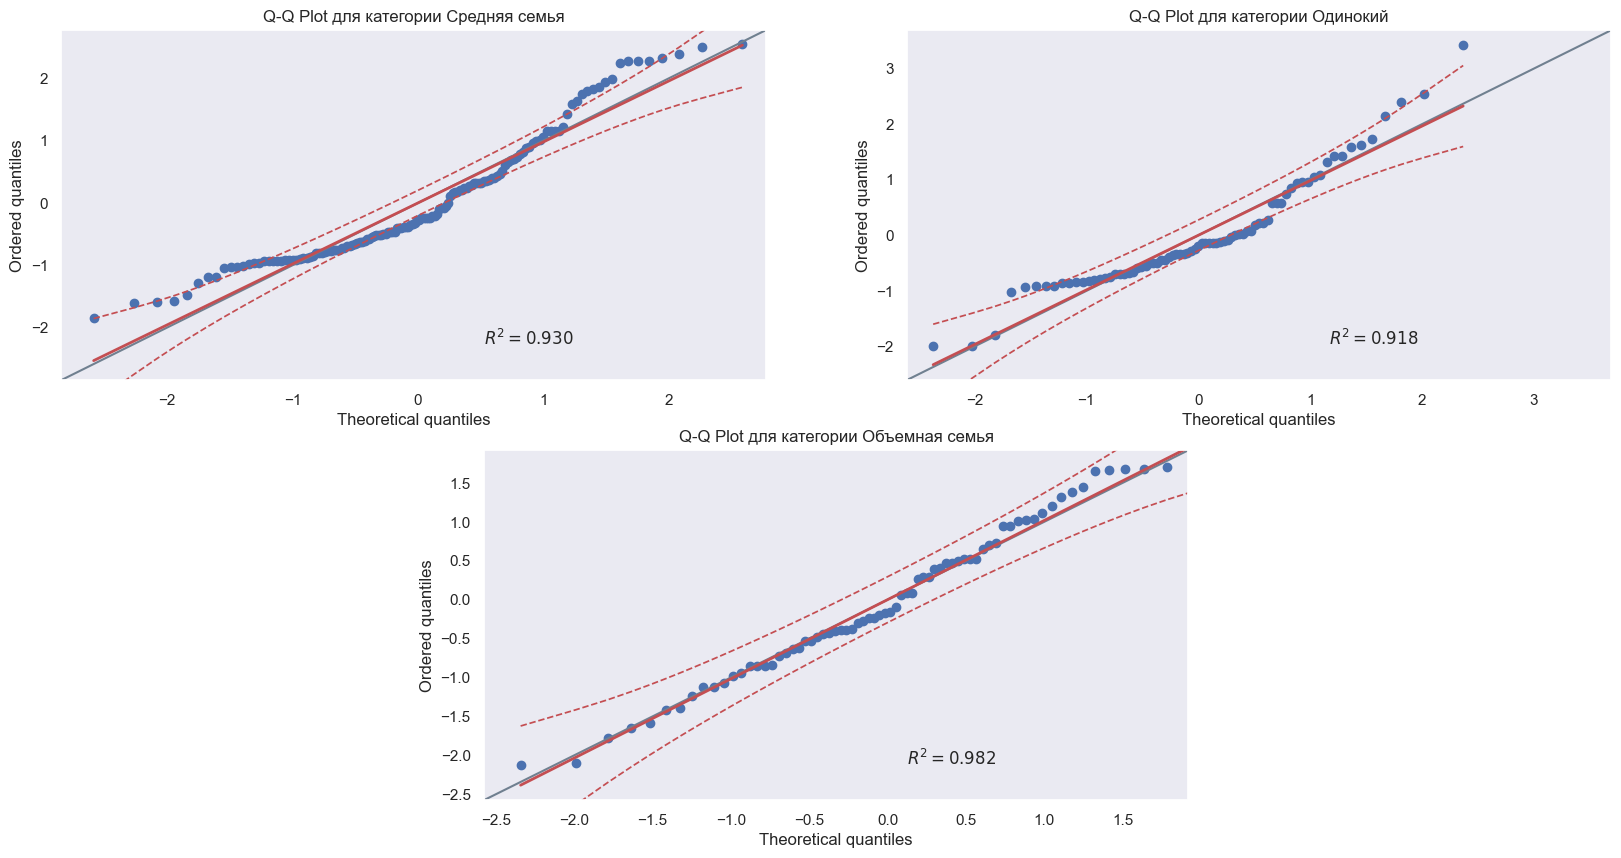
\includegraphics[scale=0.45]{title/qqplot.png}
  \caption{QQ-plots для денежных доходов по категориям}
\end{figure}
Действительно, только одна группа распределена нормально, однако стоит всё же попробовать \emph{ANOVA-test}. Проверим предварительно на гомоскедастичность (равенство дисперсий) с помощью теста Левене:
\[
    W = \dfrac{N-k}{k-1} \cdot \dfrac{\sum\limits_{i=1}^k N_i\left(Z_{i\cdot} - Z_{\cdot\cdot}\right)^2}{\sum\limits_{i=1}^k \sum\limits_{j=1}^{N_i}N_i\left(Z_{ij} - Z_{i\cdot}\right)},
\]
где $k$ -- количество групп, $N_i$ -- количество результатов исследования для $i$-ой группы, $N$ -- общее количество исследований, $Y_{ij}$ -- значение $j$-го наблюдения в $i$-ой группе.
\[
    Z_{ij} = \left|Y_{ij} - \overline{Y}_i \right|,
\]
где $\overline{Y}_i$ -- среднее по $i$-ой группе,
\[
    Z_{i\cdot} = \dfrac{1}{N_i}\sum\limits_{j=1}{N_i} Z_{ij},
\]
среднее по $Z_{ij}$ для $i$-ой группы,
\[
    Z_{\cdot\cdot} = \dfrac{1}{N}\sum\limits_{i=1}^k\sum\limits_{j=1}^{N_i} Z_{ij}
\]
среднее по всем $Z_{ij}$.
\par
В результате имеем близкое к нулю $p-$value, следовательно отклоняем гипотезу о равенстве дисперсий. Воспользуемся \emph{Welch ANOVA}, так как он более робастный по сравнению с классическим. 
\par
Имеем низкое $p$-value, следовательно отвергаем нулевую гипотезу. После отклонения нулевой гипотезы, можно выполнить апостериорный тест Геймса-Хауэлла (он устойчив к гомоскедастичности), чтобы определить, какие групповые различия являются статистически значимыми. Выясняется, что разница между одинокими людьми и большими семьями сильнее статистистически значима, чем прочая попарная разница.
\par
Второй набор гипотез
\begin{itemize}
  \item $H_0$: Средний денежный доход для многодетных ($>2$) семей не отличается от дохода малодетных ($\leq 2$);
  \item $H_1$ Средний денежный доход многодетных ($>2$) семей больше дохода малодетных ($\leq 2$).
\end{itemize}
Повторяя проверку на нормально и гомоскедастичность, получаем отклоненную гипотезу о нормальном распределении и отклоненную гипотезы о равенстве дисперсий. Воспользуемся критерием Стьюдента для проверки гипотезы о равенстве средних:
получаем практическое нулевое значение $p$-value, следовательно отвергаем гипотезу. Следовательно, возможно, что от количества детей зависит доходность семей.
\begin{figure}[H]
  \centering
  \begin{tikzpicture}[x=0.75pt,y=0.75pt,yscale=-1,xscale=1]
    %uncomment if require: \path (0,300); %set diagram left start at 0, and has height of 300
    
    %Image [id:dp9086340344894803] 
    \draw (248.05,151.05) node  {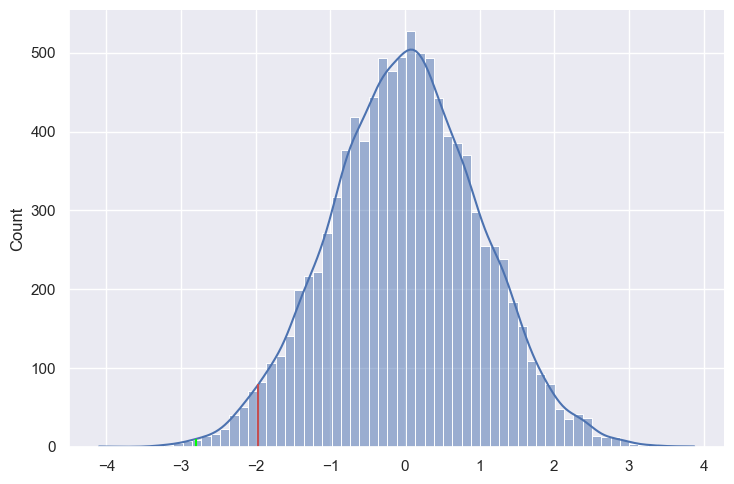
\includegraphics[width=371.89pt,height=223.39pt]{title/rejected.png}};
    %Shape: Polygon Curved [id:ds16572868611821034] 
    \draw  [draw opacity=0][fill={rgb, 255:red, 0; green, 255; blue, 0 }  ,fill opacity=1 ] (68.1,276.44) .. controls (69.92,277.51) and (133.21,271.98) .. (132.87,271.53) .. controls (132.54,271.09) and (132.87,274.53) .. (132.87,276.2) .. controls (132.87,277.87) and (66.27,275.37) .. (68.1,276.44) -- cycle ;
    
    % Text Node
    \draw (103.77,258.66) node  [font=\footnotesize] [align=left] {\begin{minipage}[lt]{45.85pt}\setlength\topsep{0pt}
    $\displaystyle p$-value
    \end{minipage}};
    % Text Node
    \draw (161.79,219.94) node  [font=\footnotesize] [align=left] {\begin{minipage}[lt]{11.72pt}\setlength\topsep{0pt}
    $\displaystyle \dfrac{\alpha }{2}$
    \end{minipage}};
    
    
    \end{tikzpicture}   
    \caption{Причины, по которой отвергаем гипотезу} 
\end{figure}
\par
Третий набор гипотез
\begin{itemize}
  \item $H_0$: Средний денежный доход равен 83100 (средний доход по Москве согласно Мосстату);
  \item $H_1$: Средний денежный доход больше 83100.
\end{itemize}
Будем использовать $t$-тест Стьюдента. Итого, имеем $p$-value равное $\approx 0.06$, значит, не отвергаем нулевую гипотезу. \vspace*{-0.64cm}

\begin{figure}[H]
  \centering
  \begin{tikzpicture}[x=0.75pt,y=0.75pt,yscale=-1,xscale=1]
    %uncomment if require: \path (0,300); %set diagram left start at 0, and has height of 300
    
    %Image [id:dp9086340344894803] 
    \draw (248.3,151.05) node  {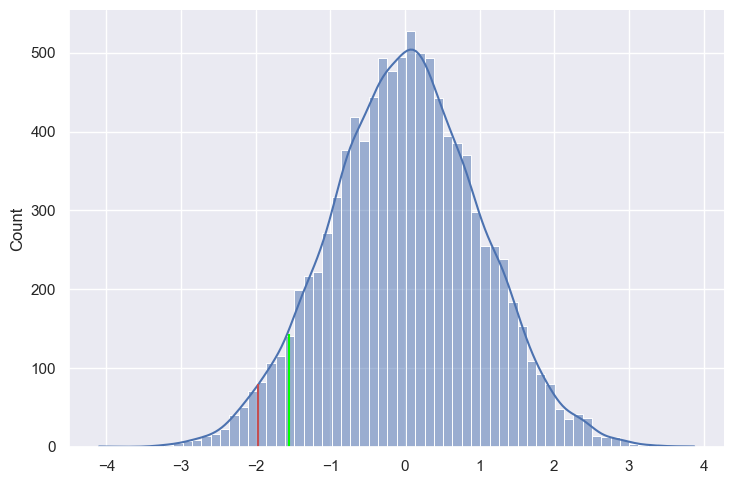
\includegraphics[width=371.89pt,height=223.39pt]{./title/not_rejected.png}};
    %Shape: Polygon Curved [id:ds16572868611821034] 
    \draw  [draw opacity=0][fill={rgb, 255:red, 0; green, 255; blue, 0 }  ,fill opacity=1 ] (68.1,276.44) .. controls (180,276.89) and (196.14,189.86) .. (195.57,207.88) .. controls (195,225.89) and (195.46,275.03) .. (195.46,276.7) .. controls (195.46,278.37) and (-43.81,275.99) .. (68.1,276.44) -- cycle ;
    %Straight Lines [id:da17054334096704138] 
    \draw [color={rgb, 255:red, 208; green, 2; blue, 27 }  ,draw opacity=1 ][line width=1.5]    (174.57,238.48) -- (174.57,276.75) ;
    
    % Text Node
    \draw (185.02,206.16) node  [font=\footnotesize] [align=left] {\begin{minipage}[lt]{45.85pt}\setlength\topsep{0pt}
    $\displaystyle p$-value
    \end{minipage}};
    % Text Node
    \draw (160.79,242.94) node  [font=\footnotesize] [align=left] {\begin{minipage}[lt]{11.72pt}\setlength\topsep{0pt}
    $\displaystyle \dfrac{\alpha }{2}$
    \end{minipage}};
    
    
    \end{tikzpicture}
    \caption{Причины, по которым не отвергаем нулевую гипотезу}
\end{figure}
\section{Взаимосвязи между признаками}
Построим матрицу корреляций (Пирсона) для количественных характеристик:
\begin{figure}[H]
  \centering
  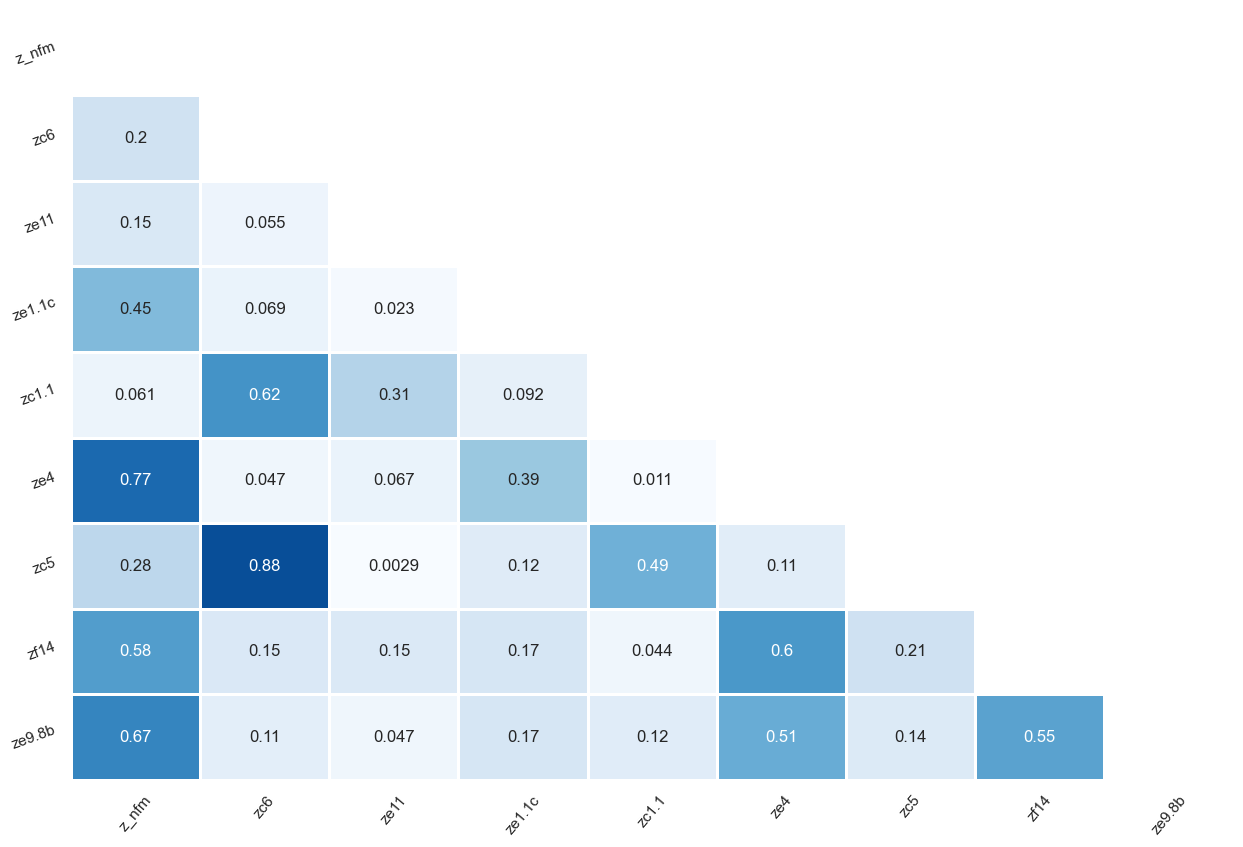
\includegraphics[scale=0.6]{title/corrlation.png}
  \caption{Heatplot для матрицы корреляций}
\end{figure}
Можно заметить очевидную зависимость между жилой и общей площадьми квартиры, а так же зависимость между количеством членов семей и их тратами на питание и мобильную связь.

\par
Построим регрессию на денежный доход, беря во внимание следующие характеристики:
\begin{itemize}
  \item[] $x_1$ -- количество членов семьи;
  \item[] $x_2$ -- примерная стоимость жилья;
  \item[] $x_3$ -- наличие иностранного автомобиля. 
\end{itemize}
Была построена регрессия по всей совокупности данных, посчитан \emph{r2\_score}.
\[
  \hat{y} = 0.3x_1 + 0.028x_2 + 0.224x_3 - 0.244x_4 + 10.1,
\]
где $x_3, x_4$ -- закодированный с помощью \emph{one-hot encoding} признак наличия иностранного автомобиля.
По критериям Шапиро-Уилка и Пирсона остатки имеют нормальное распределение на уровне надежности $0.05$. Можно сделать вывод, что примерная стоимость жилья не является значимым признаком для денежного дохода, в отличие от иностранного автомобиля и количества членов семьи. Метрика $R^2 = 0.72$.
\par 
Построим корреляции для категориальных переменных на основе критерия $\chi^2$:
\begin{figure}[H]
  \centering
  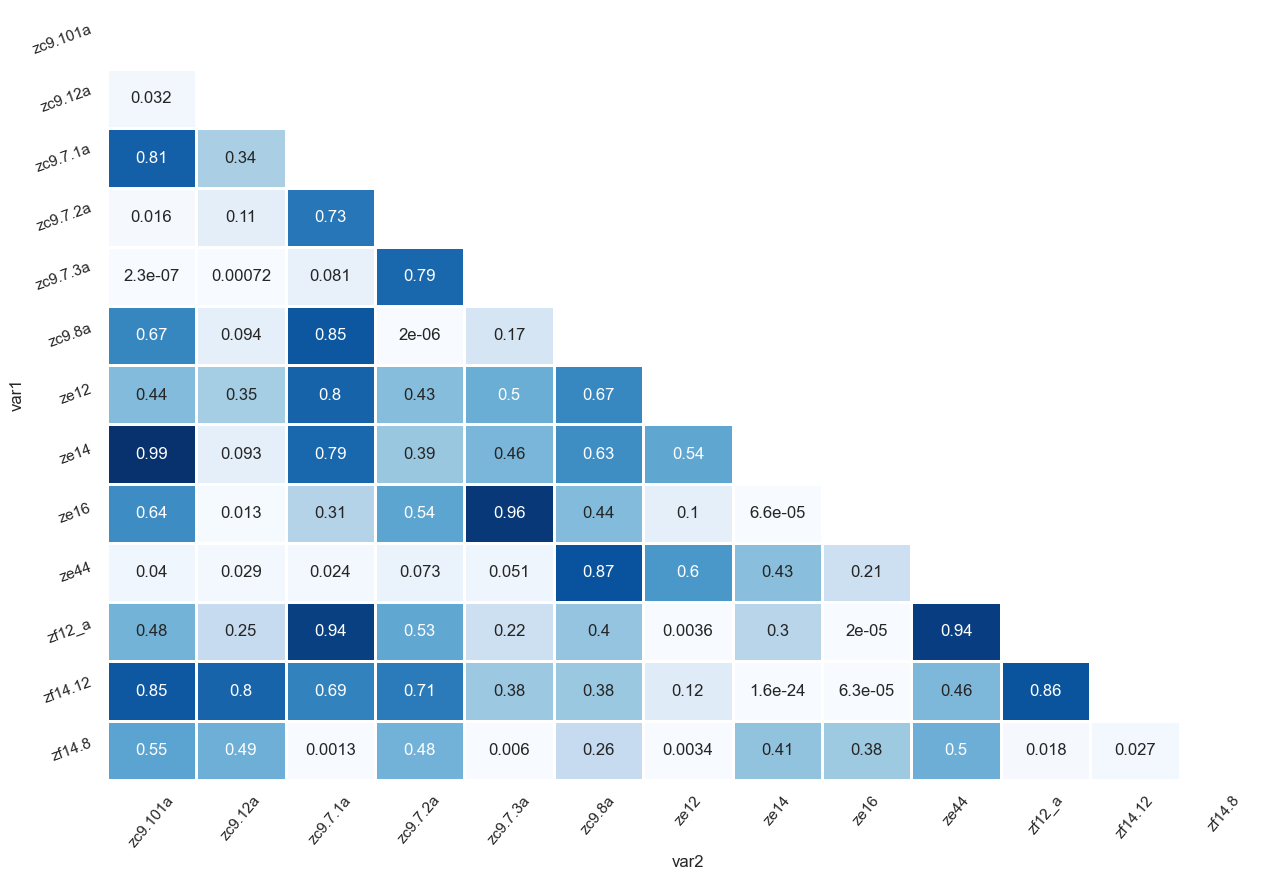
\includegraphics[scale=0.6]{title/corrlation_categorical.png}
  \caption{Heatplot для матрицы корреляций для категориальных признаков}
\end{figure}
Видны зависимости, однако они связаны с большой долей отрицательных ответов. Но, например, действительно есть зависимость между наличием иностранного автомобиля и накапливанием сбережений, $p$-value равен $\approx 0.6$ для теста на равенство частот. Рассмотрим наличие закономерности между доходами и утилизацией мусора (не самая репрезентативная с точки зрения поставленной задачи закономерность, однако интересная). Проделаем идентичные шаги, которые были в прошлом пункте. Поставим гипотезы равенства средних по группам:
\begin{itemize}
  \item[] $H_0$: В каждой группе по сортировке мусора средние по денежному доходу;
  \[
      H_0: \mu_1 = \mu_2 = \ldots = \mu_5
  \]
  \item[] $H_1$: otherwise
  \[
      H_1: \text{Все } \mu \text{ между собой не равны}
  \]
  В предикативной форме: $\exists \mu_i\ i, j \in \{1, \ldots, 5\}\ i \neq j: \ \mu_i \neq \mu_j$.
\end{itemize}
Проверим на нормальность с помощью теста Харке-Бера:
\[
    JB = n \left(\dfrac{S^2}{6} + \dfrac{(K-3)^2}{24}\right),
\]
где $\displaystyle S = \dfrac{\hat{\mu}_3}{\hat{\sigma}^3}$, $\displaystyle K = \dfrac{\hat{\mu}_{4}}{\hat{\sigma}^4}$. $p$-value $> 0.02$, на уровни значимости $0.02$ группы имеют нормальные распределения денежных доходов. Проверим гомоскедастичность методом Левене: $p$-value > $0.05$, значит, сохраняется дисперсия среди групп. Воспользуемся классическим ANOVA для получения результата: $p$-value $\approx  0.3 > \alpha \Longrightarrow $ не отвергаем гипотезу $H_0$. 
\begin{figure}[H]
  \centering
  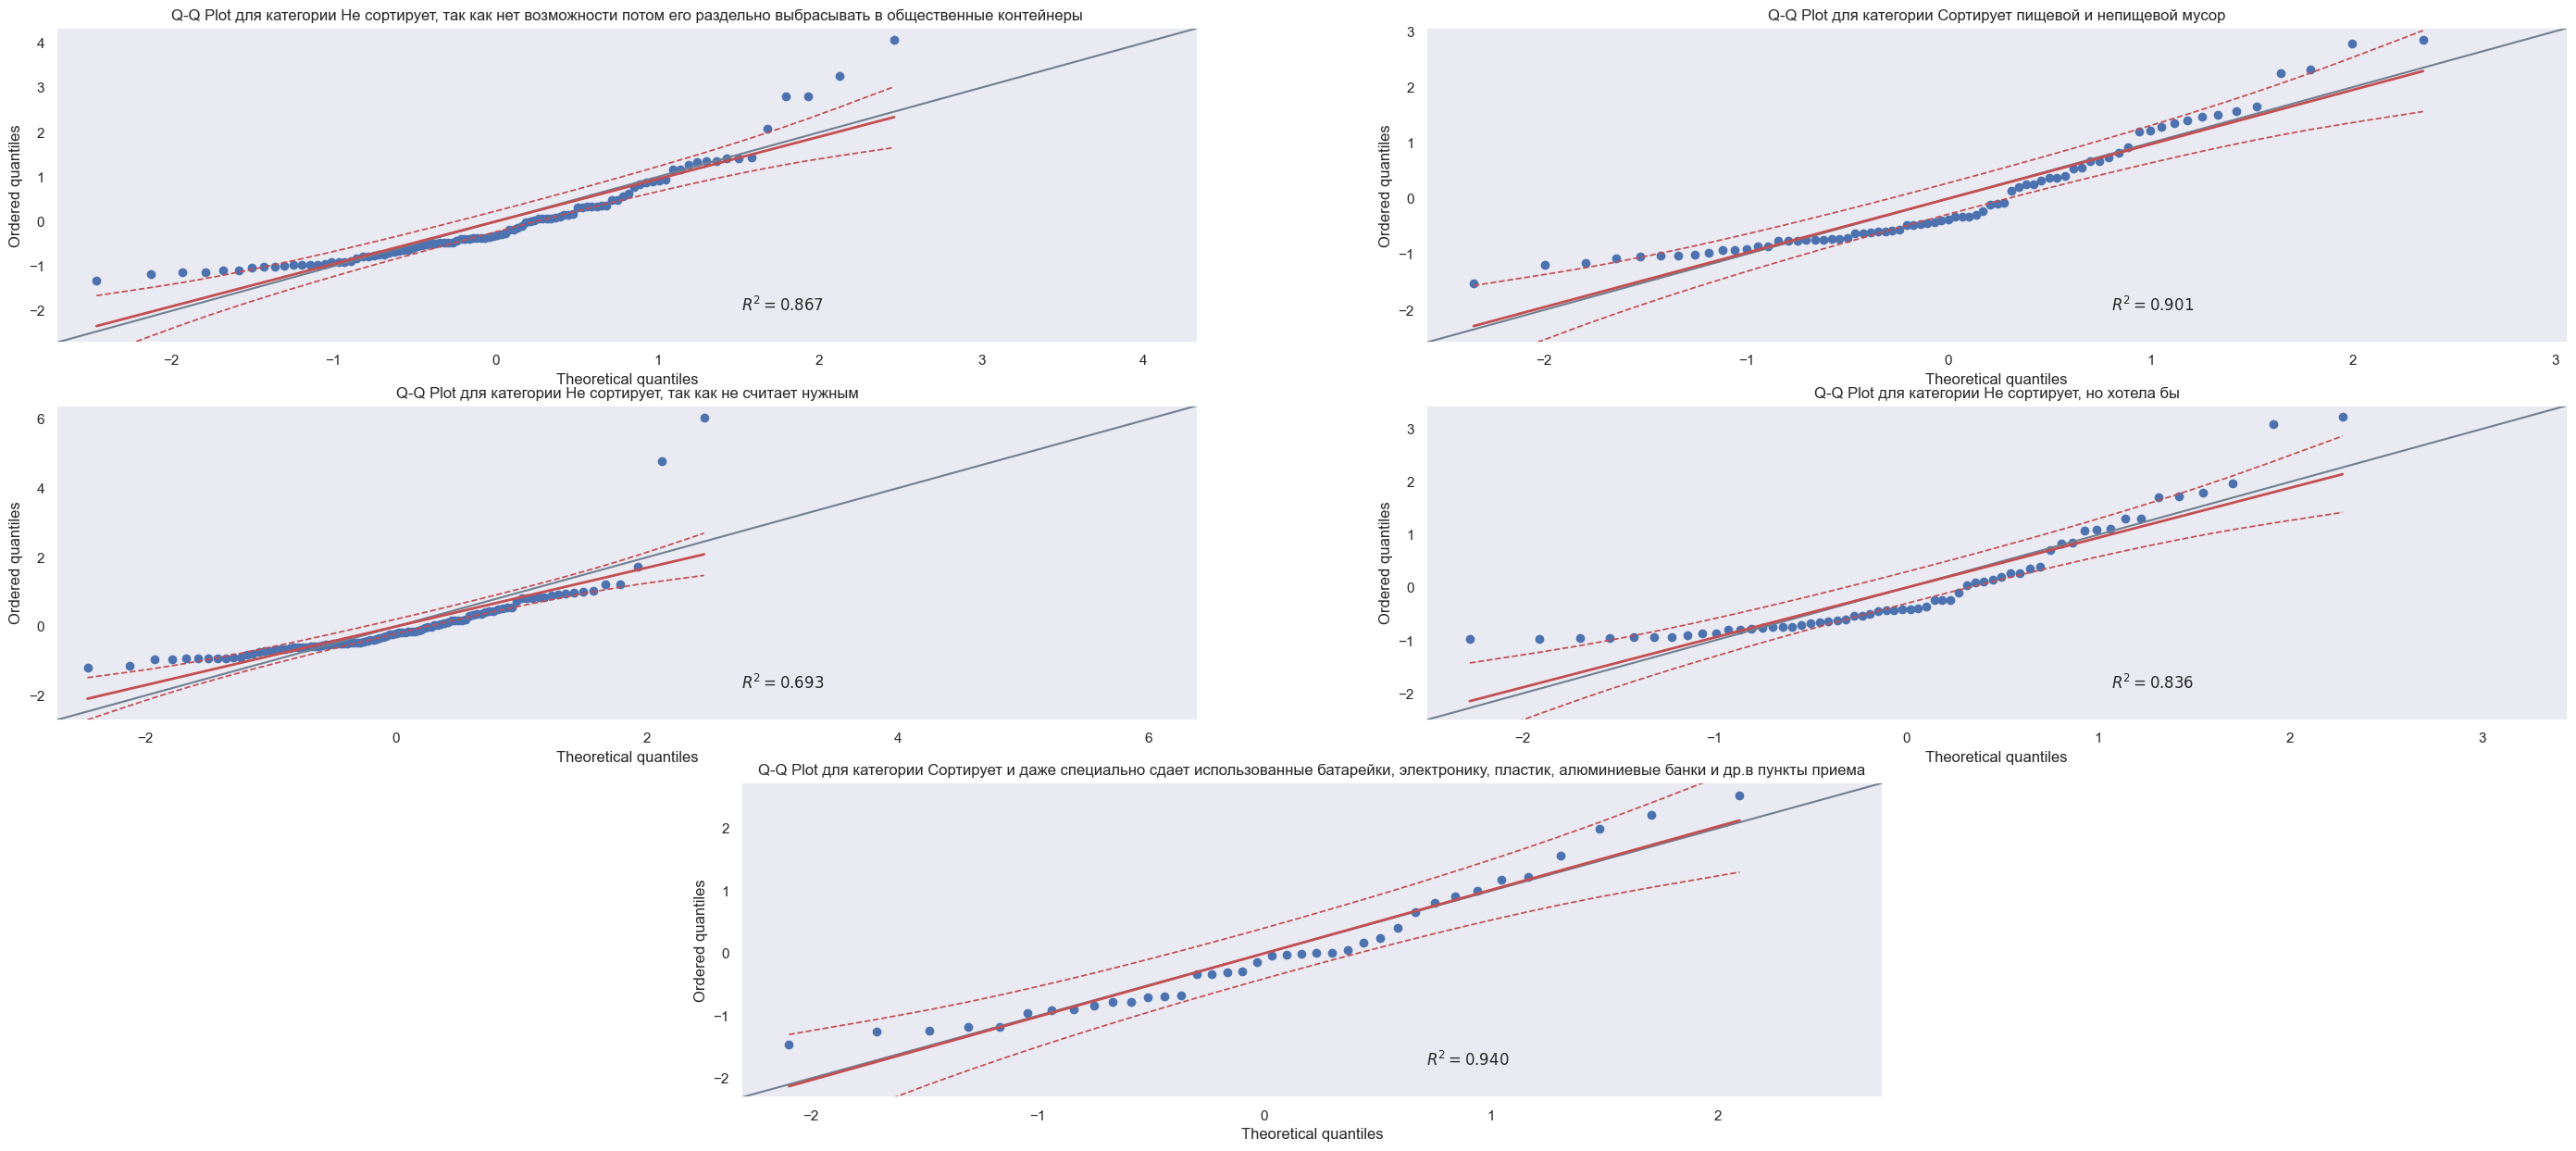
\includegraphics[scale=0.26]{title/qq_2.png}
  \caption{QQ-plots для доходов по категориям}
\end{figure} 
\end{document}
